\section{METHODS}

\subsection{Hit-and-Run algorithm}
Hit-and-Run is a method used to uniformly sample a convex \cite{smith1984efficient}, and as the set of all feasible activations is defined by the mechanics of the limb and the constraints of the task (described in \ref{ss:finger}). 
We decided to use Hit-and-run as a way to sample muscle activation solutions. 
In the case of a schematic tendon-driven limb with three muscles, the feasible activation space is the unit cube (as muscles can only be activated positively from 0 to a maximal normalized value of 1). As explained in \cite{Valero-Cuevas2009mathematical}, when task constraints are introduced to the system, the feasible activation set is further reduced; in this context, a task is a static force vector produced at the endpoint of the limb, which is represented as a set of inequality constraints. Thus if this simple limb meets all constraints, the feasible activation set of the polygon $P$ contains all feasible activation  $\textbf{a} \in \mathbb{R}^n$ that satisfy
\[\textbf{f} = A\textbf{a}, \textbf{a} \in [0,1]^n,\]
where $\textbf{f} \in \mathbb{R}^m$ is a fixed force vector and $A = J^{-T}RF_o \in \mathbb{R}^{m \times n}$---the matrices of the Jacobian of the limb, the moment arms of the tendons, and the strengths of the muscles, respectively \cite{Valero-Cuevas1998Large,Valero-Cuevas2009mathematical}. $P$ is bounded by the unit $n$-cube since all variables $a_i$, $i \in [n]$ are bounded by 0 and 1 from below, above respectively.
Consider the following $1 \times 3$ fabricated example, where the task is a 1N unidimensional force.
\begin{align*}
&1 = \frac{10}{3}a_1 - \frac{53}{15}a_2 + 2a_3 \\
&a_1, a_2, a_3 \in [0,1],
\end{align*}
the set of feasible activations is given by the shaded set in Figure \ref{fig:fig_hr}.

\begin{figure}[ht]
  \label{fig:fig_hr}
   \begin{center}
    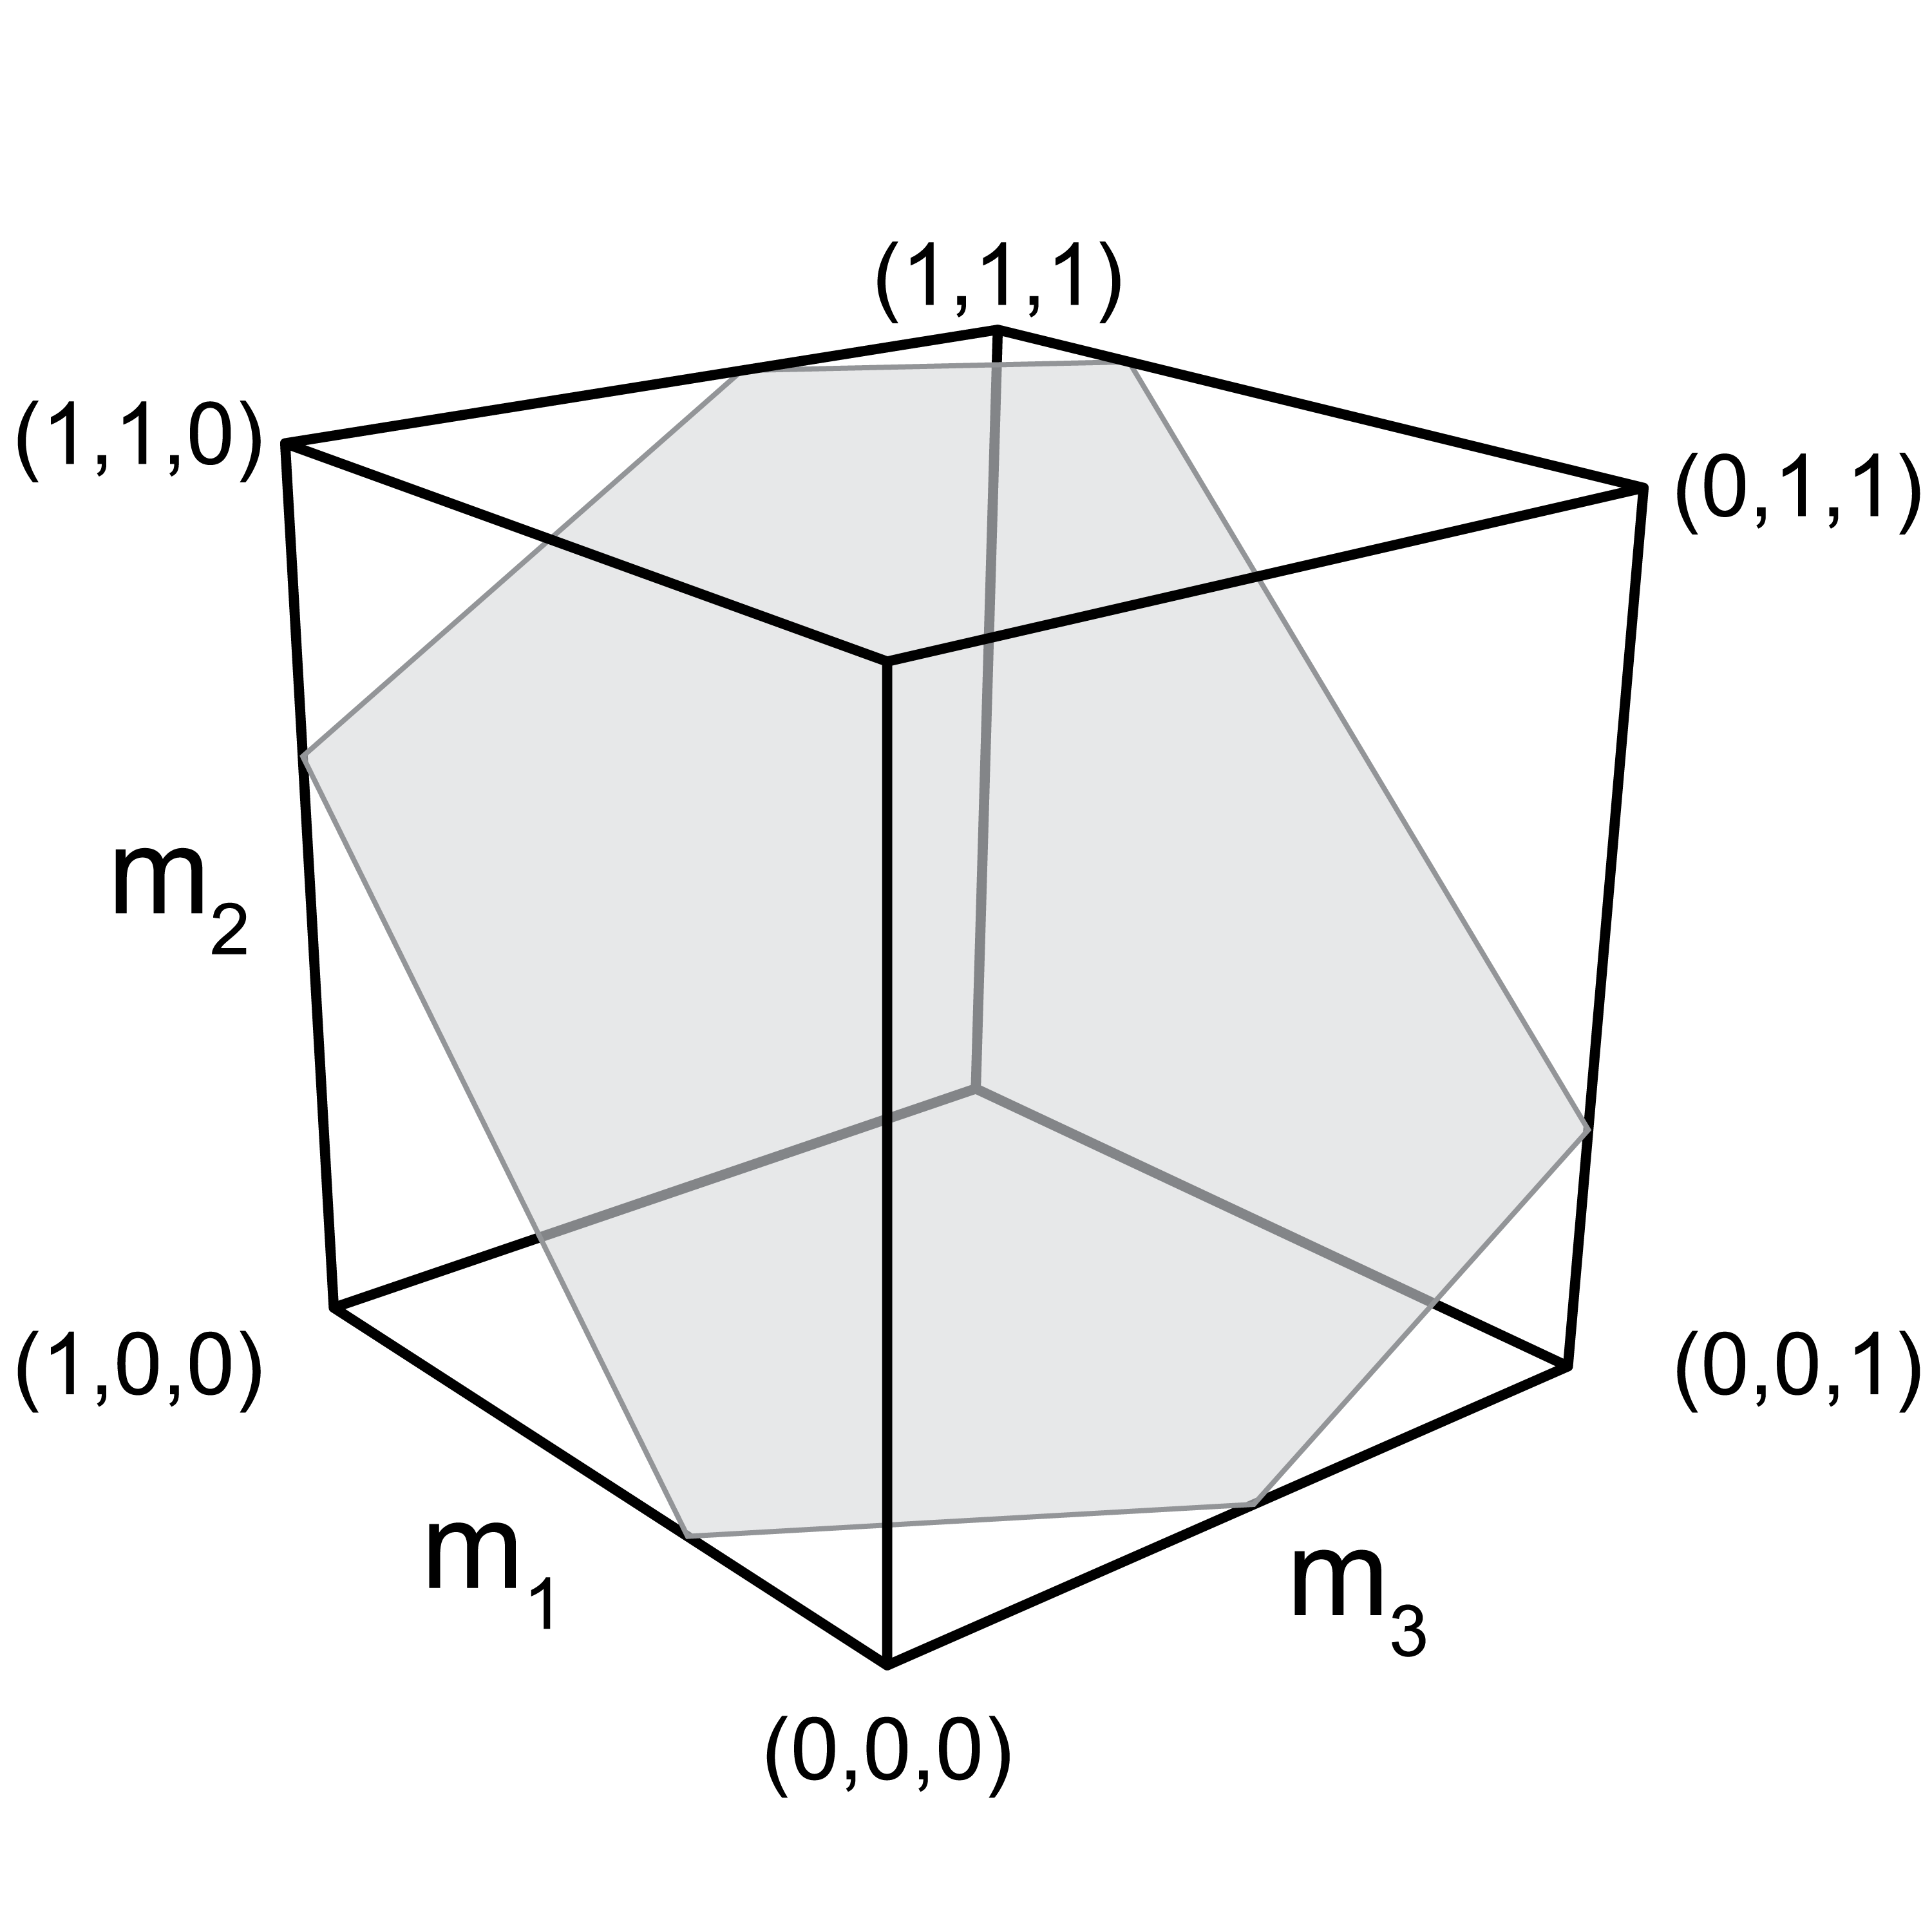
\includegraphics[width=0.25\textwidth]{sections/figs/feasibleactivation.png}
  \end{center}
  \caption{The feasible activation set for a  three-muscle system meeting one functional constraint is a polygon in $\mathbb{R}^3$. Note that muscle activations are assumed to be bounded between $0$ and $1$.}

\end{figure}

The Hit-and-Run walk on $P$ is defined as follows (it works analogously for any convex body). 
\begin{enumerate}
\item Inner Point: Find a given starting point $\textbf{p}$ of $P$ (Figure \ref{fig:hitruncube}(a)) .
\item Direction: Generate a random direction from $\textbf{p}$ (uniformly at random over all directions) (Figure \ref{fig:hitruncube}(b)).
\item Endpoints: Find the intersection points of the random direction with the edges of the polytope (Figure \ref{fig:hitruncube}(c)).
\item New Point: Pick a random distance along the line formed by the endpoints (Figure \ref{fig:hitruncube}(d)). 
\item Repeat from $(a)$ the above steps with the new point as the starting point .
\end{enumerate}


\begin{figure}[htbp]
\centering
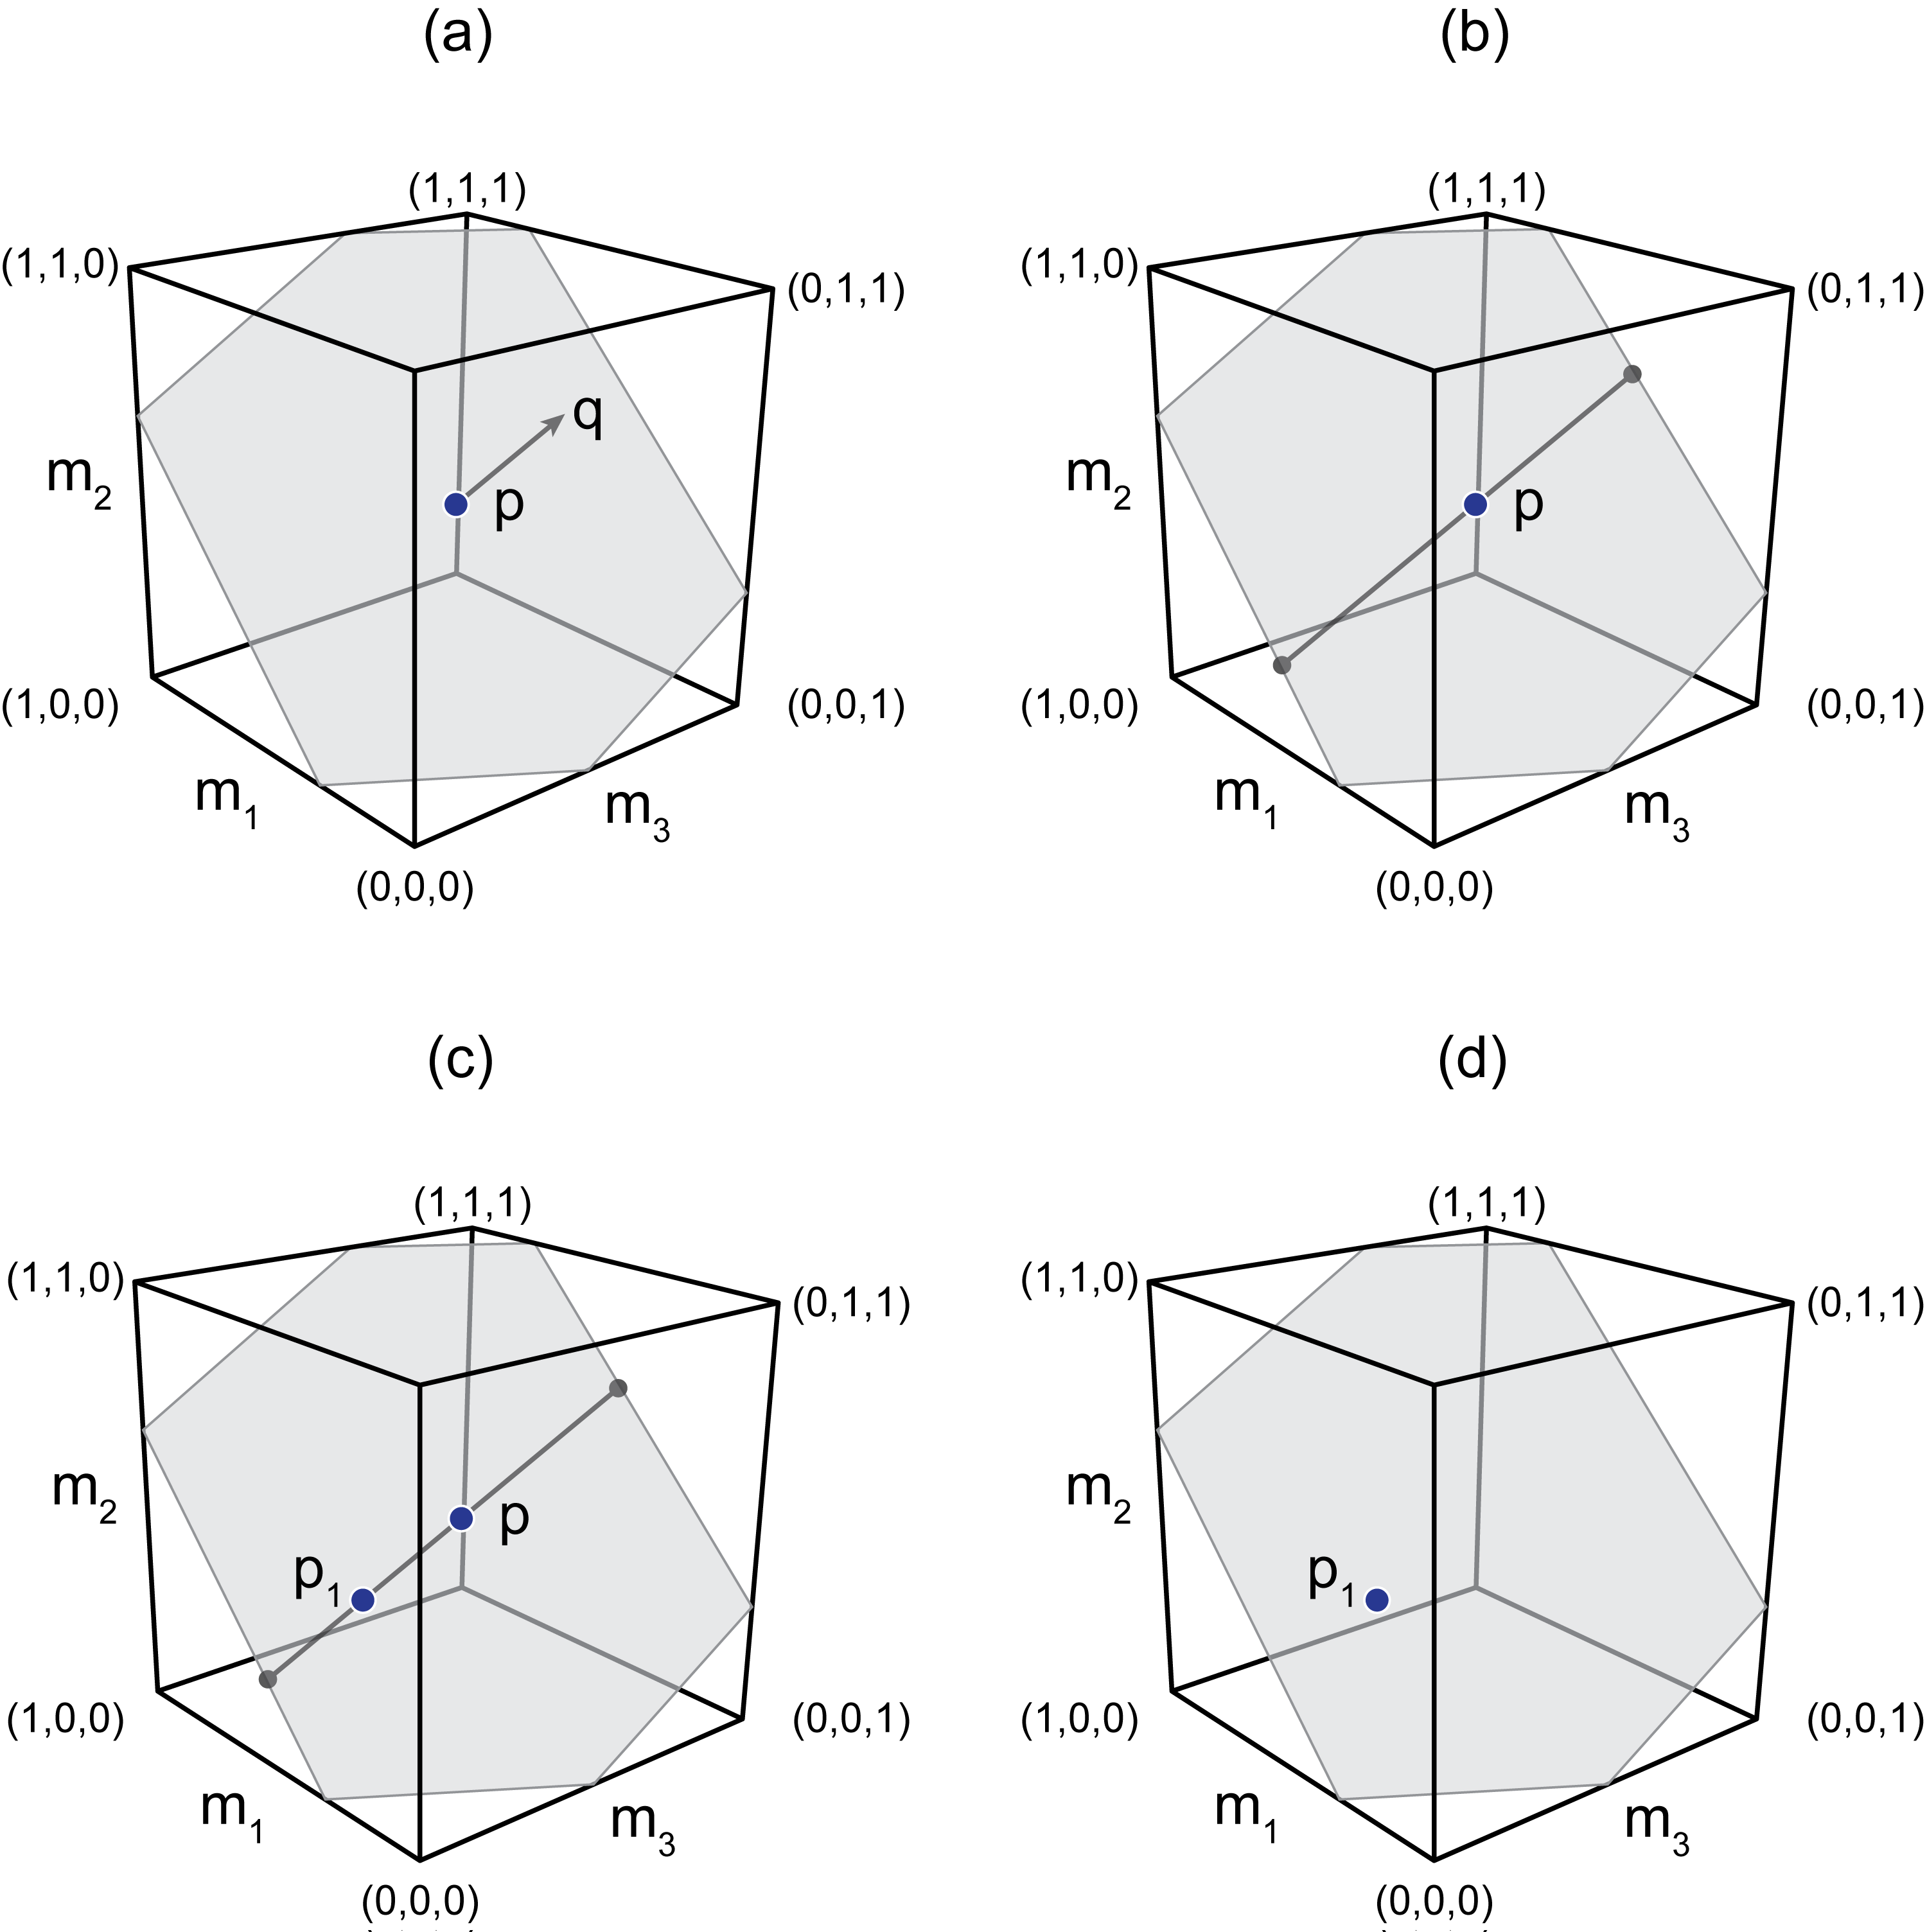
\includegraphics[width=7.5cm\textwidth]{sections/figs/hitruncube.png}
\caption{Graphical description of the Hit-and-Run algorithm.}
\label{fig:hitruncube}
\end{figure}


To find a starting point in 
\[\textbf{f} = A\textbf{a}, \textbf{a} \in [0,1]^n,\]
we only need to find a feasible activation vector. For the Hit-and-Run algorithm to mix faster, we want the starting point to be centrally located within the polytope. We use the following standard trick with slack variables $\epsilon_i$.

\begin{equation}\label{eq:LP_r}
\begin{array}{lrcl}
\mbox{maximize} & \sum_{i=1}^n \epsilon_i \\ 
\mbox{subject to} & \textbf{f} &=& A\textbf{a}\\
  & a_i &\in& [\epsilon_i, 1- \epsilon_i], \hspace{5mm} \forall i \in \{1,\dots,n\}  \\
  & \epsilon_i &\geq& 0, \hspace{5mm} \forall i \in \{1,\dots,n\}.  
\end{array}
\end{equation}

How many points are necessary to reach a uniform distribution across the polytope? For convex polygons in higher dimensions c. $40$, experimental results suggest that $\mathcal{O}(n)$ steps of the Hit-and-Run algorithm are sufficient. In particular Emiris and Fisikopoulos paper suggest that $(10 + 10\frac{n})n$ steps are enough to converge upon the uniform distribution \cite{emiris2013efficient}.
In the index finger model we executed the Hit-and-Run algorithm $1,000,000$ times.

\subsection{Realistic index finger model}
\label{ss:finger}
We used our published model in \cite{Valero-Cuevas1998Large} to find matrix $A \in \mathbb{R}^{4 \times 7}$, where $\textbf{a} \in \mathbb{R}^7$ and the four degrees of freedom were ad-abduction, flexion-extension at the metacarpophalangeal joint, and flexion-extension at the proximal and distal interphalangeal joints. The force direction we simulated is in the palmar direction in the posture shown in Figure \ref{fig:finger}.
\begin{figure}[htbp]
\centering
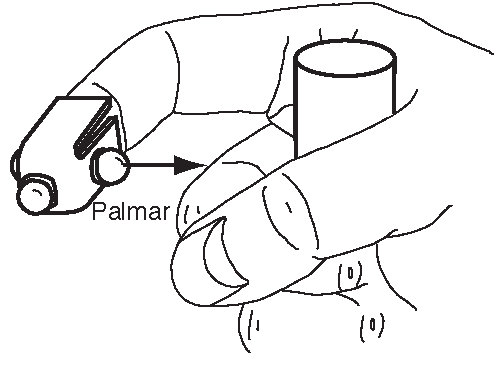
\includegraphics[width=7.5cm\textwidth]{sections/figs/finger.pdf}
\caption{The index finger model simulated 50\% of maximal force production in the palmar direction. Adapted from \cite{Valero-Cuevas1998Large}.}
\label{fig:finger}
\end{figure}


